%für Sprache, A4 Blatt, float, Grafiken, UTF Codierung, PDF, Color, Seitenabstand, Listings
\documentclass[a4papr,12pt]{article}
\usepackage[utf8]{inputenc}
\usepackage[ngerman]{babel}
\usepackage{graphicx}
\usepackage{float}
\usepackage{textcomp}
\usepackage{pdfpages}
\usepackage{tikz}
\usepackage{hyperref}
\usepackage{geometry}
\usepackage{listings}
\usepackage{color}
\usepackage{grffile}
\usepackage{caption}

%Mathematics
\usepackage{amstext}
\usepackage{amssymb}
\usepackage{amsmath}
\usepackage{amsfonts}
\usepackage{mathrsfs}
\usepackage{mathtools}

%include this before fancy or page style gets messed up bc of geometry
%Seitenabstand A4 Blatt
\geometry{a4paper}
\geometry{top=25mm,bottom=25mm,left=23mm,right=20mm}

% macro to select a scaled-down version of Bera Mono (for instance)
\makeatletter
\newcommand\BeraMonottfamily{%
  \def\fvm@Scale{0.85}% scales the font down
  \fontfamily{fvm}\selectfont% selects the Bera Mono font
}
\makeatother

%Hyperref zum anklicken von Überschriften in Texmaker + Farben einstellen
\hypersetup{
	colorlinks,
	citecolor=black,
	filecolor=black,
	linkcolor=blue,
	urlcolor=black
}

\definecolor{mygreen}{rgb}{0,0.6,0}
\definecolor{mygray}{rgb}{0.5,0.5,0.5}
\definecolor{mymauve}{rgb}{0.58,0,0.82}

%Zum Pascal Code einfügen mit lstinputlisting[language=Pascal] {../blabla.pas}
\lstset{ %
  backgroundcolor=\color{white},   % choose the background color; you must add \usepackage{color} or 								  \usepackage{xcolor}
  basicstyle=\BeraMonottfamily,        % the size of the fonts that are used for the code
  breakatwhitespace=false,         % sets if automatic breaks should only happen at whitespace
  breaklines=true,                 % sets automatic line breaking
  captionpos=b,                    % sets the caption-position to bottom
  commentstyle=\color{mygreen},    % comment style
  deletekeywords={...},            % if you want to delete keywords from the given language
  escapeinside={\%*}{*)},          % if you want to add LaTeX within your code
  extendedchars=true,              % lets you use non-ASCII characters; for 8-bits encodings only, 												does not work with UTF-8
  frame=single,	               % adds a frame around the code
  keepspaces=true,                 % keeps spaces in text, useful for keeping indentation of code 									  (possibly needs columns=flexible)
  keywordstyle=\color{blue},       % keyword style
  language=Octave,                 % the language of the code
  otherkeywords={...},           % if you want to add more keywords to the set
  numbers=left,                    % where to put the line-numbers; possible values are (none, left, 								  right)
  numbersep=5pt,                   % how far the line-numbers are from the code
  numberstyle=\tiny\color{black}, % the style that is used for the line-numbers
  rulecolor=\color{black},         % if not set, the frame-color may be changed on line-breaks within 								  not-black text (e.g. comments (green here))
  showspaces=false,                % show spaces everywhere adding particular underscores; it 														overrides 'showstringspaces'
  showstringspaces=false,          % underline spaces within strings only
  showtabs=false,                  % show tabs within strings adding particular underscores
  stepnumber=2,                    % the step between two line-numbers. If it's 1, each line will be 								  numbered
  stringstyle=\color{mymauve},     % string literal style
  title=\getlstname,
  tabsize=2,	                    % sets default tabsize to 2 spaces
  inputencoding=latin1,
  columns=fullflexible
}

\lstset{literate=%
	{Ö}{{\"O}}1
	{Ä}{{\"A}}1
	{Ü}{{\"U}}1
	{ß}{{\ss}}1
	{ü}{{\"u}}1
	{ä}{{\"a}}1
	{ö}{{\"o}}1
	{~}{{\textasciitilde}}1
}

%Filenamen und Pfad trennen
\makeatletter
\DeclareRobustCommand{\getlstname}{%
\begingroup
  % \lstname seems to change hyphens into \textendash
  \def\textendash{-}%
  \filename@parse{\lstname}%
  \texttt{\filename@base.\filename@ext}%
\endgroup
}


%Für Kopfzeile den Style
\usepackage{fancyhdr}
\pagestyle{fancy}
\lhead{AUD 2\textbackslash PRO 2 - Übung 2}
\rhead{Andreas Roither, \today{}}
\newcommand{\Cross}{\mathbin{\tikz [x=1.4ex,y=1.4ex,line width=.2ex] \draw (0,0) -- (1,1) (0,1) -- (1,0);}}%

\begin{document}

%ANGABE     
\thispagestyle{plain}
\includepdf[pages={1},pagecommand={     
\begin{tikzpicture}[remember picture, overlay]\node at (15.8, -0.85) {6 h};\end{tikzpicture}
\begin{tikzpicture}[remember picture, overlay]\node at (7.6, -0.85) {Andreas Roither};\end{tikzpicture}
\begin{Huge}
\begin{tikzpicture}[remember picture, overlay]\node at (-1.3, -1.9) {X};\end{tikzpicture}
\end{Huge}
}]{Angabe/UE2.pdf}
\thispagestyle{plain}
\includepdf[pages=2-,pagecommand={}]{Angabe/UE2.pdf}

\section*{Übung 2}
\subsection*{Aufgabe 1}
\subsubsection*{Lösungsidee}
Bei MinM wird in eine Liste eingefügt falls ein Zeichen darin noch nicht enthalten ist. Am Schluss wird gezählt wie viele Zeichen in der Liste enthalten sind. Diese Anzahl gibt MinM zurück. Bei MaxMStringLen wird solange in eine Liste eingefügt bis m erreicht wird. Falls die Anzahl unterschiedlicher Zeichen in der Liste überschritten wurde, löscht RemoveFirst das erste Zeichen in der Liste. Falls die aktuelle Länge größer ist als die vorher gespeicherte Länge wird die aktuelle Länge gespeichert.
\newline

\lstinputlisting[language=Pascal] {../Kette.pas}
\begin{figure}[H]
	\centering
	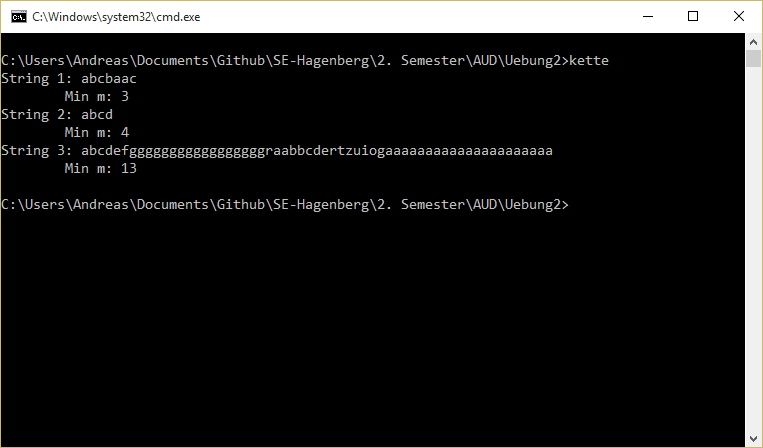
\includegraphics[scale=0.75]{./pictures/1a.png}
	\caption{Ausgabe 1a}
	\label{fig: Kette1a}
\end{figure}
Ausgegeben wird die Anzahl der unterschiedlichen Zeichen der oben angegebenen Zeichenketten.

\begin{figure}[H]
	\centering
	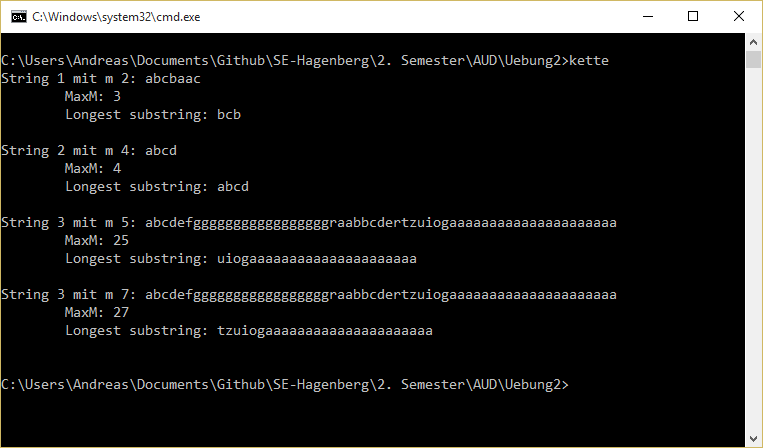
\includegraphics[scale=0.75]{./pictures/1b.png}
	\caption{Ausgabe 1b}
	\label{fig: Kette1b}
\end{figure}
Hier wird der längste Substring mit maximalen m eines Strings ausgegeben.

\newpage
\subsection*{Aufgabe 2}
\subsubsection*{Lösungsidee}
Das Matching funktioniert ähnlich wie die BruteForce Methode. Es wird von links nach rechts durch den string gegangen. Dabei wird bei jedem Aufruf ein Teil des string nicht mehr mit übergeben, für die Zeichen \grqq{}*\grqq{} und \grqq{}?\grqq{} werden dabei spezielle Aktionen durchgeführt. Falls die Zeichenfolge nicht mehr übereinstimmt wird False zurückgegeben, andernfalls wird True zurückgegeben.
\newline

\lstinputlisting[language=Pascal] {../wildcard.pas}
\begin{figure}[H]
	\centering
	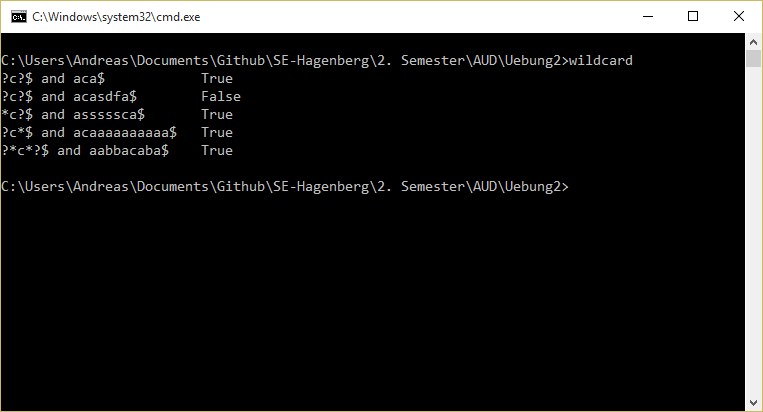
\includegraphics[scale=0.75]{./pictures/2arecursive.png}
	\caption{Ausgabe Matching}
	\label{fig: Matching}
\end{figure}
Ausgabe für die jeweiligen Zeichenketten.

\end{document}





